% Venue-neutral manuscript. To switch template: replace the preamble with elsarticle / IEEEtran /
% sn-jnl and keep \input{sections/...}. Numbers in tables/figures are generated from results/*.json.
\documentclass[11pt]{article}
\usepackage[margin=1in]{geometry}
\usepackage[T1]{fontenc}
\usepackage{lmodern}
\usepackage{amsmath,amssymb,amsthm,bm}
\usepackage{graphicx}
\usepackage{booktabs,multirow,makecell}
\usepackage{xcolor}
\usepackage[numbers,sort&compress]{natbib}
\usepackage[hidelinks]{hyperref}
\usepackage{cleveref}
\usepackage{siunitx}
\usepackage{caption,subcaption}

\newcommand{\dchi}{\Delta\chi}
\newcommand{\R}{\mathbb{R}}
\newcommand{\ESA}{ESA}
\newcommand{\SVA}{SVA}
\newcommand{\SVF}{SV-Former}
\newcommand{\ESF}{ES-Former}
\newtheorem{proposition}{Proposition}
% placeholders filled when the last runs finish (shown in red until then)
\newcommand{\NOROTSEEDS}{\textcolor{red}{[Seeds 1--2 of the no-augmentation arm pending.]}}
\newcommand{\LEAKAGE}{\textcolor{red}{[Leakage-audit numbers (DeepHerb / dual-branch reproductions, random vs.\ grouped) pending.]}}

\title{When Does Leaf Geometry Help? Sweep-Valuation Attention for\\
Studio-to-Field Medicinal Leaf Identification}
\author{Author names withheld}
\date{}

\begin{document}
\maketitle

\begin{abstract}
Medicinal-leaf classifiers report near-perfect accuracy on studio images, but little is known about
what they rely on or how they transfer to field photographs. We propose \emph{sweep-valuation
attention} (\SVA{}), a backbone-agnostic module that sweeps a leaf along many directions and, for
every slab of the sweep, measures the area and boundary length that enter a weighted cubical complex
of the blade and of a learned venation field. Each measurement becomes a token that attends to the
image patches of the same slab. We study \SVA{} against matched controls (global fusion of the same
measurements, slab attention without measurements, and strip pooling) on three backbones
(ConvNeXt-T, ViT-S, BioCLIP~2), using a de-duplicated, leaf-grouped protocol for the 30-species
Medicinal Leaf Dataset and transfer to 20 species of the DIMPSAR field photographs. Clean accuracy is
saturated for all models. With ConvNeXt-T, \SVA{} raises field-photo accuracy from 33.5\% to 49.3\%
(15/15 runs) and keeps this gain without rotation augmentation, where it exceeds strip pooling and
slab-only attention by 5--6 points. The gain disappears for ViT-S and for BioCLIP~2, which reaches
81\% without any module. Ablations show that appearance-conditioned weights and a fine sweep drive the
effect, whereas restricting attention to the slab adds little; Euler-characteristic tokens make
models sensitive to holes in the blade but transfer worse. All code, run outputs, statistics and the paper sources are available at
\url{https://github.com/Devguru-codes/research_paper_leaf}.
\end{abstract}

\section{Introduction}
\label{sec:intro}

Medicinal plants are identified in the field mostly from their leaves, and errors are not equally
costly: confusing two culinary herbs is harmless, but confusing a remedy with a toxic look-alike, such
as \textit{Nerium oleander} with other Apocynaceae, can be dangerous~\citep{farkhondeh2020oleander}.
Deep networks report 97.5--99.7\% accuracy on Indian medicinal leaf
benchmarks~\citep{roopashree2021deepherb,ffncacnn2025}. Those numbers, however, are obtained on
single leaves photographed on white backgrounds, typically with random image-level splits. They say
little about how the models behave when the same species is photographed in the field, against soil,
tiles or cloth, with a phone camera, which is where such a classifier would be used.

Botanists describe a leaf by its geometry: how wide the blade is along its length, where it tapers,
how ragged its margin is, how its veins branch. These characters are measured \emph{at particular
places} on the leaf. Standard CNN and ViT classifiers average their features over the whole image and
have no built-in notion of where the leaf is, let alone of localised geometry. A natural hypothesis is
therefore that architectures which measure leaf geometry locally, and look at the image where they
measure, should transfer better from studio to field. Recent work fuses topological and morphological
summaries with deep features~\citep{phgnet2023,tdavit2026,gu2026multifiltration,blaser2026encoding},
but usually as global descriptors, and without controls that would tell whether the geometry itself
is what helps.

We test this hypothesis with a ladder of matched models that share backbone, data, vein head and
training, and differ in one ingredient at a time: (1)~a plain classifier; (2)~the same features pooled
over the leaf mask, i.e.\ knowing \emph{where} the leaf is; (3)~localised pooling over strips of the
image or over slabs of an object-centred directional sweep; and (4)~\emph{sweep-valuation attention}
(\SVA{}), which we introduce as the most structured member of the family: for each slab of the sweep it
measures how much area and boundary length a learned, appearance-weighted cubical complex of the blade
and venation adds there, and lets that measurement attend to the image patches of the same slab. A
global fusion of the same measurements tests whether geometry helps without localisation.

The answer is clear and partly negative. On ConvNeXt-T the studio-to-field gain over a plain model
is large (14 points) but splits into two parts of similar size: knowing where the leaf is, and pooling
locally within it. Measured geometry, whether fused globally or attached to localised tokens, adds
nothing detectable. The gain is small on EfficientNet-B0, absent on a ViT, and irrelevant for a
biology foundation model, which transfers far better on its own.

\paragraph{Contributions.}
\begin{enumerate}
\item \textbf{A controlled decomposition of studio-to-field transfer} for medicinal leaves on four
  backbones, with 5 folds $\times$ 5 seeds for the main backbone, pre-specified contrasts, corrected
  resampled tests with Holm correction and a bootstrap over runs and field species. Leaf location and
  localised pooling each add 5--8 points on raw field photographs of ImageNet ConvNeXt-T; the gains
  hold without rotation augmentation and add to strong background-compositing augmentation.
\item \textbf{Sweep-valuation attention}, a differentiable, backbone-agnostic module that turns a
  directional filtration of appearance-weighted cubical complexes into slab tokens, and a careful
  negative result: its measured geometry does not improve transfer beyond localised pooling, its
  slab-restricted attention can be replaced by global attention, and Euler-characteristic tokens make
  models sensitive to topology but transfer worse.
\item \textbf{A leakage-audited protocol and probes} for the Medicinal Leaf Dataset: duplicate and
  re-shot grouping, a corruption suite (MedLeaf-C), a leaf cue-conflict set, a perceptually matched
  topology-destruction test and a verified mapping of 20 DIMPSAR field species.
\end{enumerate}
Code, splits, probes, statistics and the outputs of all training runs are released.

\section{Related work}
\label{sec:related}

\paragraph{Medicinal leaf identification.} Work on Indian medicinal leaves has moved from
hand-crafted shape, colour and texture descriptors to transfer learning. DeepHerb combined Xception
features with SVMs~\citep{roopashree2021deepherb}; later CNN, hybrid CNN--transformer and feature-fusion
models report 98.9--99.7\% on this and related datasets~\citep{ffncacnn2025}, typically with random
image-level splits. Closest to our biological motivation, a dual-branch network fuses an RGB branch
with a branch on skeletonised veins by late concatenation~\citep{dualbranch2026}. A cascaded
taxonomic classifier targets open-world medicinal plants~\citep{openworld2025medicinal}. We reproduce
DeepHerb-style and dual-branch pipelines under our leakage-audited protocol.

\paragraph{Studio-to-field shift in plant recognition.} The gap between curated and field images is
well documented for plant disease recognition: a model trained on the laboratory images of
PlantVillage reached 99.4\% on held-out laboratory images but about 31\% on images taken under
other conditions~\citep{mohanty2016plantvillage}, and the background alone of those images carries
enough signal to classify them~\citep{noyan2022plantvillagebias}. For medicinal leaves, field
evaluation is rare. We measure this gap for a medicinal leaf benchmark under a controlled protocol and
ask which architectural ingredients close it.

\paragraph{Euler characteristic transforms.} The ECT and the persistent homology transform encode a
shape through sublevel-set topology along all directions~\citep{turner2014pht}. DECT makes the ECT
differentiable by sigmoid relaxation and learns directions end-to-end~\citep{roell2024dect}. WECT
weights cells by image intensity~\citep{cisewski2023wect}. Blaser et al.\ encode the ECT as
per-direction token sequences, including convolutional and complex-valued variants that are
equivariant to planar rotations~\citep{blaser2026encoding}. For plants, Ayub et al.\ show that ECT
images of \emph{blade contours} classify complex leaf shapes and even predict venation from blade
geometry~\citep{ayub2026ectplants}. Their ECT is computed on the outline only; venation is a
prediction target, and appearance is not used. We build on DECT's relaxation and on these encodings.
We do not claim weighted, tokenised or rotation-equivariant ECTs, or ECTs of leaves, as contributions.

\paragraph{Topology meets attention.} Topological summaries are increasingly fused with deep
features. PHG-Net injects persistence-diagram features into CNN/transformer classifiers~\citep{phgnet2023};
TDA-ViT fuses topological and ViT features~\citep{tdavit2026}; GraPHFormer aligns graph topology
and vision representations~\citep{shah2026graphformer}. Gu et al.\ process multi-filtration cubical
persistence diagrams with cross-attention and fuse the embedding with CNN/transformer
features~\citep{gu2026multifiltration}. TopoFormer slices graphs along filtrations into
attention-friendly topological token sequences~\citep{uddin2026topoformer}. For time series, Faghihi and Saki add persistent-homology and directional Euler
statistics of each input window as additive biases on attention logits~\citep{faghihi2026topoattn}; the
topology summarises the whole window rather than defining where each query may attend. In these methods the
topological signal enters as a \emph{global} descriptor or as tokens among themselves, so where the
visual model looks is not tied to where the topology was measured. \SVA{} differs in exactly this
respect: each filtration slab yields both a valuation increment and the spatial support of that token's
attention. Our controls (global fusion of the same valuations; slab attention without valuations;
mask and strip pooling) separate these ingredients, and we find that the localisation, not the
measured topology or geometry, carries the effect.

\paragraph{Intrinsic volumes and directional pooling.} Area, boundary length and Euler characteristic
(the planar intrinsic volumes, or Minkowski functionals) are classical morphological descriptors with
efficient digital estimators~\citep{mecke1994,legland2007minkowski}, and the perimeter of a planar shape
can be recovered from its ECT~\citep{gacias2026convexect}; by Hadwiger's theorem they span all
continuous motion-invariant valuations~\citep{hadwiger1957,klain1997}. We use them as filtration
increments along a sweep, not as global descriptors, and do not claim them as new features. Strip
pooling~\citep{hou2020strip} and axial attention aggregate features along image rows and columns.
Our strip control instantiates this family; unlike \SVA{}, its strips are fixed to the image axes,
carry no measured geometry and are not defined by a filtration of the object.

\paragraph{Taxonomy and uncertainty.} Hyperbolic and hierarchy-aware embeddings have been applied
to plant and biological taxonomies~\citep{shah2025hprotonet,hyperbolictaxonomies2025}, and BioCLIP~2
learns hierarchical contrastive representations at scale~\citep{gu2026bioclip2}. Conformal prediction
for long-tailed plant identification~\citep{ding2026conformal} and for hierarchical
labels~\citep{hcc2025,hierarchicalcp2025} is established; we do not address uncertainty quantification
here, because the calibration data for toxic species in this dataset are too few (about ten images
per fold) for meaningful hazard-specific guarantees.

\paragraph{Shape versus texture.} ImageNet CNNs are biased towards texture~\citep{geirhos2019texture}.
We adapt the cue-conflict paradigm to leaves (silhouette of one species filled with the lamina of
another) and add a topology-destruction probe, in order to test what \SVF{} actually relies on.

\section{Data and leakage-audited protocol}
\label{sec:data}

\paragraph{Dataset.} We use the segmented subset of the Medicinal Leaf Dataset of Roopashree and
Anitha~\citep{roopashree2020dataset} (CC BY 4.0): 1{,}835 RGB photographs ($1600\times1200$) of
single leaves from 30 Indian medicinal species on a white background, with 34--122 images per
species (3.6$\times$ imbalance). The leaf covers 4.4--68.5\% of the frame (median 34.8\%). The
species span 28 genera, 19 families and 12 orders of the APG~IV system, with genuine sibling groups
(e.g.\ Apocynaceae: \textit{Nerium}, \textit{Tabernaemontana}, \textit{Carissa}; Myrtaceae:
\textit{Psidium} and two \textit{Syzygium}; Moraceae: two \textit{Ficus} and \textit{Artocarpus};
Lamiaceae: \textit{Mentha}, \textit{Ocimum}, \textit{Plectranthus}); see \cref{tab:taxonomy}.

\paragraph{Audit.} Reported accuracies on this dataset are near saturation
(97.5--99.7\%~\citep{roopashree2021deepherb,ffncacnn2025}) and use random image-level splits. Our
audit found three issues.
(i)~\emph{Exact duplicates}: 10 pairs of identical photographs saved under different names, all in
\textit{Carissa carandas} (1{,}825 images remain after removal).
(ii)~\emph{Re-shots of the same physical leaf}: some leaves were photographed more than once, at times
under different illumination or orientation. Hashing alone cannot separate these from merely similar
leaves (e.g.\ lanceolate \textit{Alpinia} silhouettes), so we link two images when their raw-frame
1024-bit dHash distance is $\le 20$, or when SIFT matching with RANSAC yields $\ge40$ geometrically
consistent inliers whose similarity transform has scale in $[0.8,1.25]$ and whose convex hull covers
$\ge25\%$ of the leaf. These criteria were set by visual inspection and reject hub matches caused by
repetitive texture (e.g.\ \textit{Mentha}). The resulting 22 multi-image groups (45 images, at most 3
per group) are kept intact across splits. Over-grouping is conservative: it constrains splits but
cannot leak.
(iii)~\emph{Filename collisions}: \textit{Psidium guajava} and \textit{Punica granatum} share the
\texttt{PG-S-xxx} prefix (65 colliding names), so files must be indexed by class and name.

\paragraph{Protocol.} All results use stratified, group-aware 5-fold cross-validation on the 1{,}825
de-duplicated images. Inside each training part, one group-aware stratified holdout ($\approx$1/6)
serves as the calibration set for conformal prediction and for monitoring only. Epoch count and
hyper-parameters are fixed in advance, with no model selection on test or calibration data. With
random image-level splits, 2--4\% of test images per fold have a duplicate or re-shot in the training
part (\cref{sec:results}).

\paragraph{Preprocessing.} The leaf mask is obtained by thresholding the white background
(all channels $<235$) followed by morphological cleaning. Each image is cropped to a square
centred on the leaf whose inscribed circle contains the whole leaf, so that any rotation about the
centre is lossless, and resized to $448^2$ (training input $384^2$). Vein pseudo-labels are
multiscale Sato ridge responses on CLAHE-normalised luminance inside the eroded mask.

\paragraph{Cross-domain test set.} For transfer to field photographs we use DIMPSAR~\citep{pushpa2023dimpsar}
(CC BY 4.0), whose single-leaf subset was captured with smartphones against varied backgrounds (tiles,
soil, cloth, paper). Vernacular folder names were mapped to species and checked visually. Twenty
species overlap ours; note that Kannada \emph{Arali} denotes \textit{Ficus religiosa} (peepal), not
\textit{Nerium oleander}. Leaves are localised with our own masker, a ConvNeXt-T FPN trained only on
our leaves composited onto DTD textures~\citep{cimpoi2014dtd} and procedural backgrounds; no
third-party segmentation model is used.

\section{Method: Sweep-Valuation Attention}
\label{sec:method}

\Cref{fig:overview} summarises \SVF{}. An appearance backbone (CNN or ViT) produces patch tokens.
Two structural fields are derived from the same image: the \emph{blade}, a deterministic leaf mask,
and a \emph{learned venation field}, a vein-probability map predicted by a light head on early backbone
features. A directional sweep partitions the leaf into ordered slabs. For every direction--slab pair,
\SVA{} measures how much of each field's \emph{intrinsic volumes} (area and boundary length) enters
the filtration inside that slab, and uses \emph{the same slab} to restrict where the resulting token
attends among the patch tokens.

\begin{figure*}[t]
\centering
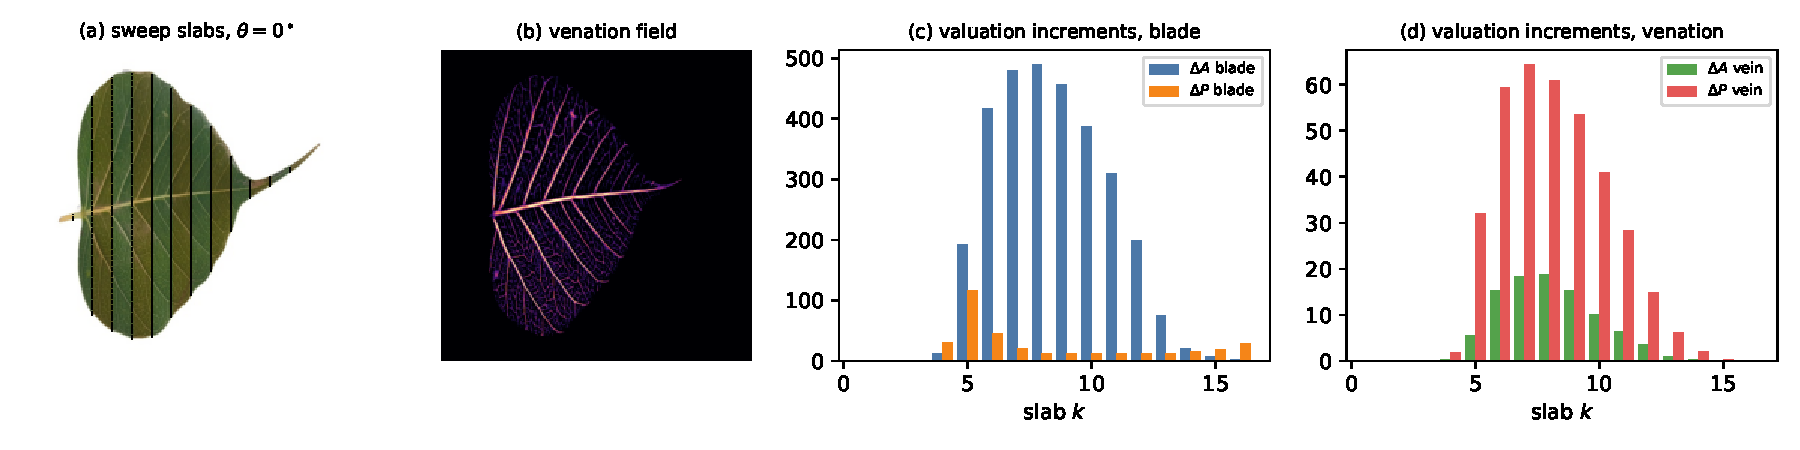
\includegraphics[width=\textwidth]{figures/fig_overview.pdf}
\caption{The sweep-valuation signal for one leaf (\textit{Ficus religiosa}) and one of the $K{=}32$
directions. (a)~The leaf is partitioned into $T{=}16$ slabs along $\theta$ in its centroid/RMS frame.
(b)~Ridge-filter vein pseudo-label that supervises the learned venation field. (c,d)~Area and
perimeter increments per slab for the blade and the venation field, shown here with unit weights; in
\SVA{} the cell weights are appearance-conditioned. Each slab's increments form the query of one
token, which attends to the image patches of the same slab. The long perimeter in the last blade
slabs comes from the drip tip.}
\label{fig:overview}
\end{figure*}
\subsection{Weighted cubical complexes}
The leaf crop is resampled to a $G\times G$ grid ($G{=}96$). Pixel centres $x_p$ are expressed in
a frame centred at the blade centroid and scaled by its root-mean-square radius, which makes all
quantities below invariant to translation and isotropic scale. We use the cubical complex whose
0-cells are pixels, whose 1-cells are pairs of 4-adjacent pixels and whose 2-cells are $2\times2$
pixel squares. Given per-pixel weights $a(p)\in[0,1]$, cells inherit the minimum weight of their
vertices,
\begin{equation}
  w_0(p)=a(p),\qquad w_1(e)=\min_{v\in e}a(v),\qquad w_2(q)=\min_{v\in q}a(v).
  \label{eq:weights}
\end{equation}
This keeps face monotonicity $w(\text{coface})\le w(\text{face})$, so the weighted complex is a fuzzy
subcomplex. For binary $a$ it reduces exactly to the standard cubical complex of the set.

\paragraph{Appearance-conditioned weights.} Two weight fields are built from mid-level backbone
features $f$ (bilinearly sampled at the grid), a small per-pixel MLP $g$ and a sigmoid $\sigma$:
\begin{equation}
 a_{\mathrm{b}}(p) = m(p)\,\sigma\!\big(g_{\mathrm{b}}(f(p))\big),\qquad
 a_{\mathrm{v}}(p) = m(p)\,v(p)\,\sigma\!\big(g_{\mathrm{v}}(f(p))\big),
\end{equation}
where $m$ is the blade mask and $v$ is the predicted vein probability. The last layer of $g$ is
initialised so that $a\approx 0.88\,m$ at the start of training. The vein head is pseudo-supervised
by a multiscale Sato ridge response~\citep{sato1998ridge} inside the eroded mask and also receives
task gradients through \SVA{}. In contrast to fixed intensity weights (WECT~\citep{cisewski2023wect}),
the weights are learned and conditioned on appearance. We stress that $a_{\mathrm{v}}$ is a
\emph{learned} venation field, not an observed vascular structure.

\subsection{Valuations of a weighted cubical complex}
Let $H_d=\sum_{c\in C_d}w_d(c)$ be the weighted number of $d$-cells. For a binary set the three
quantities
\begin{equation}
 A = H_2,\qquad P = 2H_1-4H_2,\qquad \chi = H_0-H_1+H_2
 \label{eq:valuations}
\end{equation}
are the area (number of unit squares), the boundary length in pixel units (every square contributes
four edges, and an edge shared by two squares is interior) and the Euler characteristic. They are
the cubical counterparts of the three planar intrinsic volumes. By Hadwiger's
theorem~\citep{hadwiger1957,klain1997}, every continuous, rigid-motion-invariant valuation on planar
convex bodies is a linear combination of these three. Because~\eqref{eq:valuations} is linear in the
cell weights, it extends directly to the fuzzy complex~\eqref{eq:weights}. Our proposed token uses
area and perimeter, i.e.\ the two \emph{metric} intrinsic volumes. The purely topological one, $\chi$,
is retained as an ablation (\cref{sec:abl}), because in our pilots it did not add information beyond
area and perimeter (\cref{sec:results}).

\subsection{Filtration increments along a sweep}
For a direction $\theta\in S^1$ we use the lower-star filtration,
$h_\theta(v)=\langle x_v,\theta\rangle$ and $h_\theta(c)=\max_{v\in c}h_\theta(v)$. Following the
sigmoid relaxation of DECT~\citep{roell2024dect}, a cell enters the filtration at threshold $t$ with
soft indicator $\sigma(\lambda(t-h_\theta(c)))$. Fix thresholds $t_0<t_1<\dots<t_T$, where
$t_1,\dots,t_{T-1}$ are uniform on $(-R,R)$, $t_0=-\infty$ and $t_T=+\infty$. The soft membership of
height $h$ in slab $k$ is
\begin{equation}
 s_k(h)=\sigma\big(\lambda(t_k-h)\big)-\sigma\big(\lambda(t_{k-1}-h)\big),\qquad k=1,\dots,T,
 \label{eq:slab}
\end{equation}
and because the outer thresholds are infinite, $\sum_k s_k(h)=1$ for every $h$. The
\emph{filtration increment} of the weighted $d$-cell count in slab $k$ is
$\Delta H_d(\theta,k)=\sum_{c\in C_d}w_d(c)\,s_k(h_\theta(c))$, and the valuation increments follow by
linearity:
\begin{equation}
 \Delta A(\theta,k)=\Delta H_2,\qquad \Delta P(\theta,k)=2\Delta H_1-4\Delta H_2,\qquad
 \dchi(\theta,k)=\Delta H_0-\Delta H_1+\Delta H_2 .
 \label{eq:increment}
\end{equation}
Each is the change of the corresponding relaxed valuation of the sublevel set between $t_{k-1}$ and
$t_k$, and $\sum_k$ telescopes to the total valuation of the leaf, independently of $\theta$. We
compute~\eqref{eq:increment} for the blade ($a_{\mathrm b}$) and the venation field ($a_{\mathrm v}$)
with $K$ uniform directions and $T$ slabs ($K{=}32$, $T{=}16$, $R{=}2$, $\lambda=\kappa T/2R$ with
$\kappa{=}4$).

\paragraph{Sweep-valuation token.} The structural feature of token $(\theta,k)$ is the 8-vector of
area and perimeter increments of both fields together with their cumulative values up to slab $k$,
\begin{equation}
 \phi(\theta,k)=\operatorname{slog}\Big[\Delta A_{\mathrm b},\Delta P_{\mathrm b},\Delta A_{\mathrm v},
 \Delta P_{\mathrm v},\ \textstyle\sum_{j\le k}(\cdot)\Big],\qquad \operatorname{slog}(x)=\operatorname{sign}(x)\log(1+|x|).
\end{equation}
The increments describe the local width profile and boundary complexity of the slab; the cumulative
values locate it within the leaf. The Euler variant replaces $\phi$ by
$[\dchi_{\mathrm b},\dchi_{\mathrm v},\chi_{\mathrm b}(t_k),\chi_{\mathrm v}(t_k)]$, and the Hadwiger
variant uses all three valuations (12 features).

\paragraph{Efficient computation.} Directions are fixed and coordinates come from the mask, so the
heights carry no gradient; only the weights do. We hard-bin heights into $n_b{=}256$ fine bins,
scatter-add cell weights per dimension into a per-direction histogram, and apply the slab
kernel~\eqref{eq:slab} evaluated at bin centres with one matrix product (the kernel is built in
double precision). This costs $O(BKN)$ memory for $N$ cells, needs no sorting, and is exact in the
telescoping and sharp limits (verified by unit tests, \cref{app:tests}).

\subsection{Co-registered slab attention}
Each direction--slab pair $(\theta,k)$ defines one sweep token with query
$q_{\theta k}=\mathrm{MLP}(\phi(\theta,k))+e_k$, where $e_k$ is a learned slab-index embedding. The token
cross-attends to the backbone patch tokens $\{z_p\}$ with an additive bias derived from the
\emph{same} soft slab membership~\eqref{eq:slab}, evaluated at patch centres:
\begin{equation}
 \mathrm{attn}_{(\theta,k)}(p)\propto\exp\!\Big(\tfrac{\langle W_Q q_{\theta k},\,W_K z_p\rangle}{\sqrt{d}}
 +\log\!\big(s_k(\langle x_p,\theta\rangle)\,\bar m(p)+\epsilon\big)\Big),
 \label{eq:attn}
\end{equation}
where $\bar m(p)$ is the fraction of leaf pixels in patch $p$ and $\epsilon=10^{-4}$. The structural
measurement and the visual evidence attached to it are thus taken over the same filtration-defined
region. To the best of our knowledge, we did not find prior work that explicitly co-registers
filtration-derived valuation increments with attention restricted to the corresponding filtration
slab (\cref{sec:related}). The attention output is added to the query with a mass gate
$M/(M+0.5)$, $M=\sum_p s_k\bar m$, so that slabs outside the leaf contribute little. The $KT{=}512$
tokens are mixed by a two-layer \emph{sweep transformer} whose learned relative position bias depends
only on $(\Delta\theta \bmod K,\Delta k)$. Tokens are mean-pooled and concatenated with the backbone's
global token for classification. Training minimises cross-entropy (label smoothing $0.1$) plus
$0.2\times$ the masked BCE of the vein head.

\subsection{Symmetry properties}
\begin{proposition}\label{prop:equiv}
Let $\mathcal R$ be a rotation by a multiple of $90^\circ$ acting on the pixel grid and let the
weights be unit (binary blade). Then $\Delta A$, $\Delta P$ and $\dchi$ of $\mathcal R I$ equal
those of $I$ cyclically shifted by $K/4$ along $\theta$ for each multiple of $90^\circ$; for
rotations by $2\pi/K$ the same holds up to grid resampling.
\end{proposition}
\noindent The proof follows from $\langle \mathcal R x,\theta\rangle=\langle x,\mathcal R^{-1}\theta\rangle$,
the equivariance of the centroid/RMS frame, and the fact that a $90^\circ$ grid rotation maps cells
of each dimension bijectively onto cells of the same dimension (so the counts $H_d$ in every slab are
permuted, not changed). It is checked numerically in \cref{app:tests}. The appearance-conditioned
weighted signal and the full \SVF{} inherit the rotation behaviour of the backbone
($f(\mathcal R I)\neq\mathcal R f(I)$ in general). We therefore do \emph{not} claim exact invariance
for them and evaluate their behaviour empirically (\cref{sec:results}). Rotation-equivariant
ECT tokenisation as such is not our contribution~\citep{blaser2026encoding}.

\subsection{Controls built from the same code}
\label{sec:controls}
To isolate what matters, we compare five models that share the backbone, vein head, training recipe
and, where applicable, the token width and transformer depth:
\begin{enumerate}
 \item \textbf{plain}: backbone global token only;
 \item \textbf{global}: the full $K\times T\times8$ valuation grid flattened through an MLP and fused
   globally (in the spirit of~\citep{phgnet2023,gu2026multifiltration}); same structural content,
   no co-registration;
 \item \textbf{strip}: strip pooling~\citep{hou2020strip}, i.e.\ mask-weighted means of patch tokens
   over every row and column of the patch grid, with learned positions and the same two-layer
   transformer; localised directional pooling without an object-centred sweep or structural content;
 \item \textbf{slab-only}: identical to \SVA{} except that $\phi\equiv0$, so each query is only the slab
   embedding $e_k$; the same co-registered slab geometry, no valuation content;
 \item \textbf{\SVA{}} (proposed).
\end{enumerate}
Model 2 versus 5 asks whether co-registration matters; 3 versus 5 asks whether an object-centred
filtration sweep matters beyond generic directional pooling; 4 versus 5 asks whether the measured
valuations matter beyond the slab geometry itself.

\section{Experimental setup}
\label{sec:experiments}

\paragraph{Backbones and training.} The main backbones are ConvNeXt-T (ImageNet-1k), ViT-S/16
(AugReg, ImageNet-21k$\to$1k) and the BioCLIP~2 ViT-L/14 visual tower (all but the last two blocks
frozen). All variants of a backbone share the recipe: AdamW (new modules lr $10^{-3}$, weight decay
$0.05$), 2 warm-up epochs then cosine decay, batch 32, mixed precision, label smoothing $0.1$. The
backbone lr is $10^{-4}$ for ConvNeXt-T and $5\times10^{-5}$ for ViT-S, both trained 40 epochs at
$384^2$; BioCLIP~2 uses lr $3\times10^{-5}$, 20 epochs and $224^2$ input. Inputs are converted to
each backbone's own normalisation statistics. Augmentation uses uniform
rotation in $[-180^\circ,180^\circ]$, scale $[0.85,1.15]$, translation $\pm5\%$, horizontal flips and
mild colour jitter. Geometric transforms are applied jointly to image, mask and vein pseudo-label. No
early stopping or test-time augmentation is used. Runs use Kaggle T4 GPUs.

\paragraph{Metrics and statistics.} We report accuracy, balanced accuracy, macro-F1, expected
calibration error (15 bins) and \emph{mistake severity}, i.e.\ the mean taxonomic distance (1 = same
genus \ldots\ 4 = different order) between predicted and true species over errors. All splits are
grouped stratified 5-fold cross-validation over the deduplicated, leaf-grouped data (\cref{sec:data}).
For ConvNeXt-T the five models are trained with 3 seeds per fold (15 runs each); the full probe suite
is run on seed 0 and the cross-domain test on all seeds. ViT-S and BioCLIP~2 use one seed per fold.
Ablations use ConvNeXt-T, seed 0, folds 0--2. Paired comparisons use the Wilcoxon signed-rank test
over fold--seed pairs and McNemar's test on pooled predictions.

\paragraph{Ablations.} Starting from \SVA{}: Euler-only and full-Hadwiger tokens; blade-only and
vein-only fields; unit cell weights; \emph{permuted} learned weights (the same weight values shuffled
within the leaf before computing the valuations, which keeps their distribution but destroys the
weight--location correspondence); global instead of slab-restricted attention; a coarser sweep
($K{=}16$, $T{=}8$); and a softer or sharper relaxation ($\kappa\in\{1,16\}$). A separate arm trains
plain, strip, slab-only and \SVA{} on all folds and three seeds \emph{without} rotation augmentation,
to measure robustness that is built in rather than learned from data.

\paragraph{Mechanistic probes.} All probes are applied to each fold's test images with fixed seeds.
\begin{itemize}
\item \textbf{Rotation sweep}: accuracy at $0^\circ,30^\circ,\dots,330^\circ$ and the fraction of
images whose prediction is identical at all 12 angles.
\item \textbf{MedLeaf-C}: ten corruptions $\times$ three severities: Gaussian noise, blur, JPEG,
low resolution, darkening, contrast loss, hue shift (yellowing), desaturation (severity 3 is
grayscale), occluders, and pasted procedural/soil-like backgrounds. Masks are the oracle masks
transformed consistently.
\item \textbf{Cue conflict}: the silhouette of a test leaf $A$ is filled with the lamina of a test
leaf $B$ of another species. $B$ is aligned by principal axes and enlarged until it covers $A$, so
that $B$'s outline contributes no shape cue. Shape bias $=n_A/(n_A+n_B)$ where $n_A$ ($n_B$) counts
predictions of $A$'s ($B$'s) species. We also report it on pairs with anisotropic stretch $\le2$.
\item \textbf{Topology destruction}: appearance-preserving edits that change topology versus matched
controls that do not. For the blade: three interior holes (exact $\Delta\chi=-3$, verified) versus
three boundary bites of equal removed area ($\Delta\chi=0$, verified). For venation: inpainting eight
small disks on strong veins versus eight on vein-free lamina. Every edit records LPIPS, pixel RMSE and
a colour-histogram distance. The response (KL divergence between clean and edited predictions) is
analysed by regression on visual distance with a topology-changing indicator.
\item \textbf{Cross-domain}: models trained on the segmented images are tested on the 20 overlapping
DIMPSAR species, both on auto-masked crops with the background whitened and on raw crops with the
background kept (30-way and 20-way-restricted accuracy).
\end{itemize}

\section{Results}
\label{sec:results}

All numbers below are generated from the run outputs by the released scripts; $\pm$ is the standard
deviation over runs. Differences are given as mean over matched fold--seed runs, with the number of
runs in which the first model wins and 95\% intervals as described in \cref{sec:experiments}.

\begin{table*}[t]
\centering
\caption{Main results (\%). Clean = in-domain grouped 5-fold accuracy; Rot.\ min = worst accuracy over
12 rotations; MedLeaf-C = mean over 10 corruptions $\times$ 3 severities; Shape bias from the
cue-conflict set; Field = 20-way accuracy on DIMPSAR field photographs (auto-masked or raw).
ConvNeXt-T: 5 folds $\times$ 5 seeds (MedLeaf-C: seeds 0, 3, 4, all seeds for mask pooling; Rot.\ min
and shape bias: seed 0); EfficientNet-B0: 5 folds
$\times$ 3 seeds; ViT-S and BioCLIP~2: 5 folds, one seed. Mask pooling was run on ConvNeXt-T only.}
\label{tab:main}
\small
\resizebox{\textwidth}{!}{\begin{tabular}{llcccccc}
\toprule
Backbone & Model & Clean & Rot.\ min & MedLeaf-C & Shape bias & Field (mask) & Field (raw) \\
\midrule
ConvNeXt-T & Plain & 99.9\,$\pm$\,0.1 & 99.9\,$\pm$\,0.2 & 81.1\,$\pm$\,1.1 & 6.5\,$\pm$\,1.5 & 35.1\,$\pm$\,1.3 & 33.5\,$\pm$\,1.2 \\
 & Global fusion & 100.0\,$\pm$\,0.1 & 99.7\,$\pm$\,0.3 & 81.0\,$\pm$\,0.8 & 7.0\,$\pm$\,1.9 & 34.9\,$\pm$\,1.7 & 33.7\,$\pm$\,1.3 \\
 & Strip pooling & 100.0\,$\pm$\,0.0 & 99.9\,$\pm$\,0.1 & 87.6\,$\pm$\,0.8 & 9.1\,$\pm$\,1.5 & 42.9\,$\pm$\,1.6 & 47.8\,$\pm$\,2.0 \\
 & Slab-only & 100.0\,$\pm$\,0.1 & 100.0\,$\pm$\,0.0 & 89.4\,$\pm$\,0.9 & 7.4\,$\pm$\,1.9 & 42.2\,$\pm$\,1.1 & 45.7\,$\pm$\,2.0 \\
 & SVA (ours) & 100.0\,$\pm$\,0.1 & 99.9\,$\pm$\,0.1 & 88.6\,$\pm$\,0.5 & 9.0\,$\pm$\,2.3 & 43.1\,$\pm$\,2.8 & 49.3\,$\pm$\,2.8 \\
\midrule
ViT-S/16 & Plain & 99.9\,$\pm$\,0.1 & 99.9\,$\pm$\,0.1 & 96.4\,$\pm$\,0.3 & 9.7\,$\pm$\,1.0 & 51.6\,$\pm$\,0.4 & 60.4\,$\pm$\,0.9 \\
 & Global fusion & 100.0\,$\pm$\,0.0 & 99.9\,$\pm$\,0.1 & 96.2\,$\pm$\,0.6 & 9.1\,$\pm$\,1.3 & 50.1\,$\pm$\,0.7 & 58.6\,$\pm$\,1.8 \\
 & Strip pooling & 99.9\,$\pm$\,0.1 & 99.9\,$\pm$\,0.1 & 96.2\,$\pm$\,0.5 & 10.3\,$\pm$\,1.3 & 51.2\,$\pm$\,1.1 & 62.7\,$\pm$\,1.0 \\
 & Slab-only & 100.0\,$\pm$\,0.0 & 99.8\,$\pm$\,0.1 & 96.6\,$\pm$\,0.5 & 11.0\,$\pm$\,1.4 & 52.0\,$\pm$\,0.8 & 64.8\,$\pm$\,2.1 \\
 & SVA (ours) & 99.9\,$\pm$\,0.1 & 99.9\,$\pm$\,0.1 & 96.6\,$\pm$\,0.3 & 9.3\,$\pm$\,1.8 & 51.9\,$\pm$\,1.0 & 60.7\,$\pm$\,1.4 \\
\midrule
BioCLIP 2 & Plain & 99.9\,$\pm$\,0.1 & 99.0\,$\pm$\,0.4 & 93.8\,$\pm$\,0.5 & 14.0\,$\pm$\,1.3 & 58.9\,$\pm$\,0.5 & 81.4\,$\pm$\,0.7 \\
 & Global fusion & 99.9\,$\pm$\,0.1 & 99.0\,$\pm$\,0.4 & 93.8\,$\pm$\,0.6 & 14.3\,$\pm$\,2.3 & 59.7\,$\pm$\,1.1 & 81.3\,$\pm$\,0.2 \\
 & Strip pooling & 99.9\,$\pm$\,0.1 & 99.2\,$\pm$\,0.5 & 93.8\,$\pm$\,0.2 & 14.2\,$\pm$\,1.7 & 58.9\,$\pm$\,0.7 & 81.5\,$\pm$\,0.5 \\
 & Slab-only & 100.0\,$\pm$\,0.0 & 98.8\,$\pm$\,0.5 & 93.9\,$\pm$\,0.6 & 13.9\,$\pm$\,1.2 & 60.7\,$\pm$\,0.7 & 81.8\,$\pm$\,1.4 \\
 & SVA (ours) & 100.0\,$\pm$\,0.0 & 98.5\,$\pm$\,0.5 & 93.5\,$\pm$\,0.5 & 13.7\,$\pm$\,2.0 & 59.8\,$\pm$\,1.1 & 81.7\,$\pm$\,0.8 \\
\bottomrule
\end{tabular}}
\end{table*}

\subsection{In-domain accuracy is saturated}
On the de-duplicated, grouped protocol every model on every backbone reaches 99.9--100\% clean
accuracy and $\ge98.5\%$ accuracy under any rotation (\cref{tab:main}). The studio benchmark therefore
cannot separate architectures, and none of the added modules costs clean accuracy. All further
results concern robustness and, primarily, transfer to field photographs.

\subsection{Decomposing the studio-to-field gain}
\label{sec:decomp}
\Cref{fig:crossdomain} and \cref{tab:contrasts} show the main result. A plain ConvNeXt-T trained on
studio images reaches 33.6\% on raw field photographs. The localised models reach 45.7--47.4\%, a gain
of 12--14 points. The ladder of matched models splits this gain into two parts of similar size.

\emph{Leaf location.} Pooling the same patch features over the leaf mask raises raw field accuracy to
41.1\% ($+7.5$ points, 25/25 runs, Holm $p<10^{-4}$), and masked-photo accuracy by $+5.7$. The plain
model averages features over the whole photograph, and on field photographs the background (tiles,
soil, cloth) is a large part of it; a model that knows where the leaf is can ignore it.

\emph{Localisation.} Pooling locally within the leaf adds a further 4.6--6.2 points on raw photographs:
strip pooling $+5.7$ (25/25, Holm $p=0.002$), slab-only attention $+4.6$ (24/25, Holm $p=0.008$) and
\SVA{} $+6.2$ (23/25; Holm $p=0.18$ because its run-to-run variance is the largest). The two-way
bootstrap over runs and field species excludes zero for all three. On masked photographs, where the
background is already removed, localisation adds only 1.2--1.6 points (not significant).

\emph{Measured geometry.} Adding the measured valuations to localised tokens does not help detectably.
\SVA{} is tied with strip pooling ($+0.5$, 12/25) and with its own slab-only variant ($+1.7$, 16/25),
with intervals of roughly $\pm4$ points around these values. Fusing the same valuations globally,
without localisation, gives no gain at all over plain ($-0.1$, 13/25). Object-centred sweep slabs
and image-axis strips perform the same.

\begin{figure}[t]
\centering
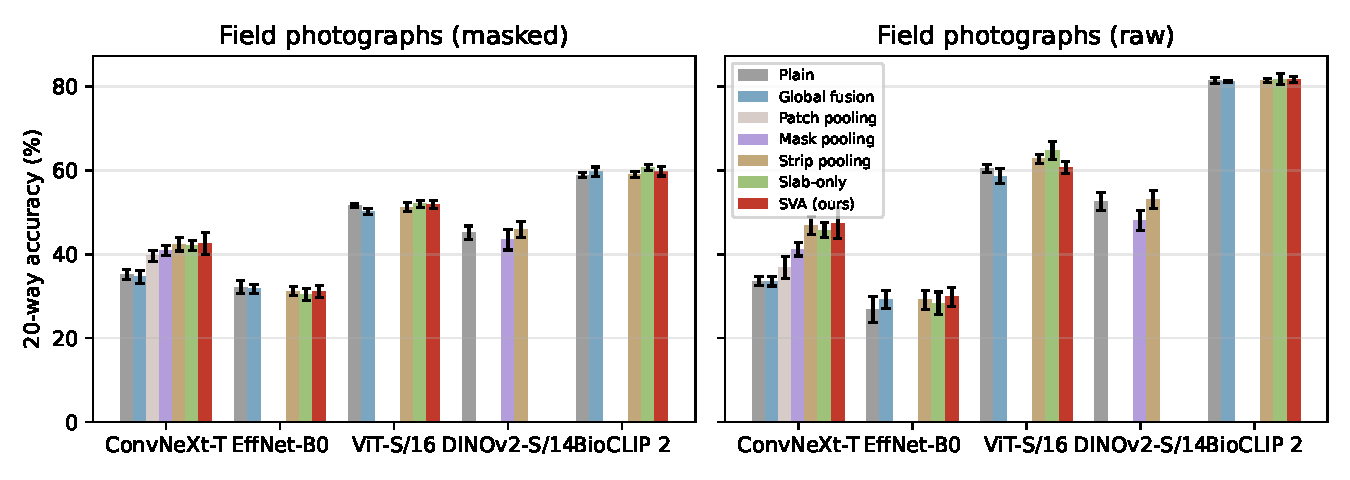
\includegraphics[width=\linewidth]{figures/fig_crossdomain.pdf}
\caption{Studio-to-field transfer: 20-way accuracy on DIMPSAR photographs with the background
whitened by our masker (left) or kept (right). Error bars: std over runs. Mask pooling was run on
ConvNeXt-T only.}
\label{fig:crossdomain}
\end{figure}

\begin{table}[t]
\centering
\caption{Pre-specified contrasts on field photographs (ConvNeXt-T, 25 matched runs). $\Delta$ in
accuracy points with runs won; 95\% intervals from the corrected resampled $t$-test over runs and from
a bootstrap over runs and field species; $p$ Holm-corrected over all 14 contrasts.}
\label{tab:contrasts}
\small
\resizebox{\linewidth}{!}{\begin{tabular}{llcccc}
\toprule
Photos & Contrast & $\Delta$ (points) & 95\% CI, runs & 95\% CI, runs+species & Holm $p$ \\
\midrule
raw & mask pooling $-$ plain & +7.5 (25/25) & [+5.3, +9.8] & [+3.0, +12.2] & $<10^{-4}$ \\
 & strip $-$ mask pooling & +5.7 (25/25) & [+3.0, +8.4] & [+2.3, +9.2] & 0.002 \\
 & slab-only $-$ mask pooling & +4.6 (24/25) & [+2.1, +7.0] & [+0.7, +8.9] & 0.008 \\
 & SVA $-$ mask pooling & +6.2 (23/25) & [+1.2, +11.3] & [+2.4, +10.2] & 0.18 \\
 & SVA $-$ slab-only & +1.7 (16/25) & [-3.5, +6.8] & [-2.8, +6.5] & 1.00 \\
 & SVA $-$ strip & +0.5 (12/25) & [-3.6, +4.7] & [-3.0, +4.5] & 1.00 \\
 & global fusion $-$ plain & -0.1 (13/25) & [-1.5, +1.3] & [-2.3, +2.4] & 1.00 \\
\midrule
masked & mask pooling $-$ plain & +5.7 (25/25) & [+3.6, +7.8] & [+2.3, +9.3] & 0.000 \\
 & strip $-$ mask pooling & +1.5 (21/25) & [-0.7, +3.7] & [-1.4, +4.3] & 1.00 \\
 & slab-only $-$ mask pooling & +1.2 (20/25) & [-0.7, +3.2] & [-2.4, +5.0] & 1.00 \\
 & SVA $-$ mask pooling & +1.6 (17/25) & [-1.7, +4.9] & [-1.7, +4.9] & 1.00 \\
 & SVA $-$ slab-only & +0.4 (15/25) & [-3.2, +3.9] & [-3.4, +4.4] & 1.00 \\
 & SVA $-$ strip & +0.1 (15/25) & [-3.4, +3.5] & [-2.9, +3.4] & 1.00 \\
 & global fusion $-$ plain & -0.6 (8/25) & [-2.4, +1.2] & [-3.4, +2.3] & 1.00 \\
\bottomrule
\end{tabular}}
\end{table}

\subsection{The gains are not an artefact of augmentation}
\label{sec:norot}
\label{sec:strongaug}
\emph{Without rotation augmentation} (5 folds $\times$ 5 seeds), the localised models remain far more
rotation-robust than plain (worst-case accuracy 97.5--98.4\% vs.\ 93.2\%; \cref{fig:rotation}) and
keep their field gain: plain 32.1\%, slab-only 43.2\%, strip 43.9\%, \SVA{} 45.5\% on raw photographs
(\SVA{} vs.\ plain $+13.5$ [$+9.7$, $+17.3$], 25/25). \SVA{} is again not distinguishable from strip
pooling ($+1.6$, 16/25) or slab-only attention ($+2.4$, 20/25). With a single seed these leads had
looked much larger ($+5.8$ and $+5.2$), which illustrates why we rely on many seeds.

\emph{With strong augmentation} (background compositing, blur, noise; \cref{tab:strongaug}), every
model improves: plain rises from 33.6\% to 42.0\% on raw photographs, about as much as mask pooling
gives without it, which is consistent with both teaching the model to discount the background.
Localisation still adds on top: strip pooling reaches 53.4\% and \SVA{} 55.2\%, the best field
accuracy of any ImageNet model here (\SVA{} vs.\ plain $+13.2$ [$+9.9$, $+16.5$], 15/15; vs.\ strip
$+1.9$, 13/15, n.s.). The architectural and data-side remedies are therefore complementary.

\begin{figure}[t]
\centering
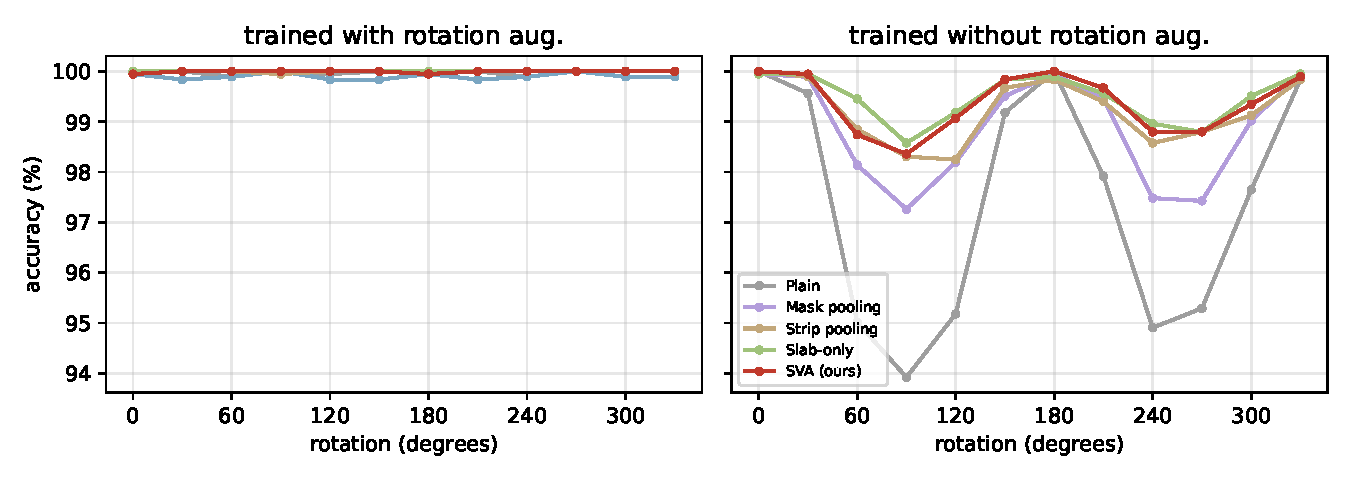
\includegraphics[width=\linewidth]{figures/fig_rotation.pdf}
\caption{Accuracy versus test-time rotation (ConvNeXt-T, seed 0, mean over 5 folds), trained with
(left) and without (right) rotation augmentation.}
\label{fig:rotation}
\end{figure}

\begin{table}[t]
\centering
\caption{Standard vs.\ strong (background compositing + blur + noise) augmentation, ConvNeXt-T,
5 folds $\times$ 3 seeds, \%.}
\label{tab:strongaug}
\small
\begin{tabular}{llccc}
\toprule
Augmentation & Model & MedLeaf-C & Field (mask) & Field (raw) \\
\midrule
standard & Plain & 81.1\,$\pm$\,1.1 & 35.1\,$\pm$\,1.3 & 33.5\,$\pm$\,1.2 \\
 & Strip pooling & 87.6\,$\pm$\,0.8 & 42.9\,$\pm$\,1.6 & 47.8\,$\pm$\,2.0 \\
 & SVA (ours) & 88.6\,$\pm$\,0.5 & 43.1\,$\pm$\,2.8 & 49.3\,$\pm$\,2.8 \\
\midrule
strong & Plain & 96.5\,$\pm$\,0.3 & 43.1\,$\pm$\,1.3 & 42.0\,$\pm$\,1.7 \\
 & Strip pooling & 97.9\,$\pm$\,0.1 & 49.3\,$\pm$\,1.3 & 53.4\,$\pm$\,1.7 \\
 & SVA (ours) & 97.8\,$\pm$\,0.3 & 49.4\,$\pm$\,1.7 & 55.2\,$\pm$\,2.0 \\
\bottomrule
\end{tabular}
\end{table}

\subsection{The gains depend on the backbone}
On EfficientNet-B0 (3 seeds) all four structural models gain only 1.5--3 points on raw photographs
(plain 26.8\%, \SVA{} 29.8\%, $+3.0$ [$-2.6$, $+8.6$], 11/15) and nothing on masked ones. On ViT-S,
localised pooling may still help (strip 62.7\%, slab-only 64.8\% vs.\ plain 60.4\%, one seed), but
\SVA{} does not (60.7\%). BioCLIP~2 reaches 81.4\% on raw photographs without any module, about
30 points above the best ImageNet ConvNeXt-T model, and all variants lie within 0.5 points of each
other. A biology foundation model thus closes most of the studio-to-field gap on its own. For both
ViTs, masked photographs are 8--22 points \emph{harder} than raw ones, whereas for the CNNs the two
differ by at most about five points; the whitened background and the masker's errors apparently remove context these models
use, so we treat raw photographs as the primary field test.

\subsection{Corruptions and cue conflict}
On MedLeaf-C (\cref{fig:corruptions}), the ladder repeats on ConvNeXt-T: mask pooling improves on plain
by $+2.7$ points (84.8\% vs.\ 82.1\%, 15/15), and localised pooling adds a further 2.2--4.0 (strip
87.5\%, \SVA{} 87.0\%, slab-only 88.8\%). The gains come from noise, blur, JPEG and low-resolution
corruptions, i.e.\ from degraded texture; colour, occlusion and background corruptions are near
ceiling for all models. On the other backbones all variants are within about one point. Shape bias
remains low everywhere (7--14\%): when a silhouette is filled with another species' lamina, all models
mostly follow the lamina. Localised pooling raises ConvNeXt-T shape bias only slightly (plain 6.5\%,
strip 9.1\%, \SVA{} 9.0\%), and BioCLIP~2 is the most shape-biased backbone (14\%). The localised
models are therefore not shape-based; they are less brittle under texture degradation and domain
shift.

\begin{figure}[t]
\centering
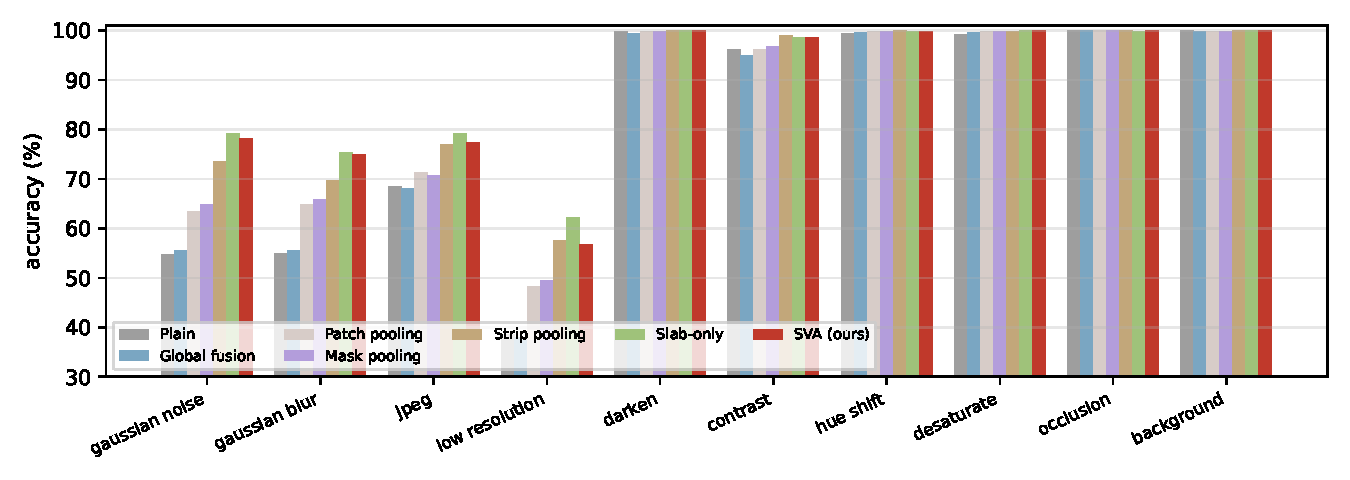
\includegraphics[width=\linewidth]{figures/fig_corruptions.pdf}
\caption{MedLeaf-C accuracy per corruption family (ConvNeXt-T, severity-averaged).}
\label{fig:corruptions}
\end{figure}

\subsection{Inside \SVA{}: ablations}
\label{sec:abl}
\Cref{tab:abl} varies one ingredient of \SVA{} at a time (ConvNeXt-T). A single-seed screen on folds
0--2 (lower block) was followed by the four most informative ablations on all 5 folds $\times$ 3
seeds (upper block), compared with \SVA{} on the same runs. The screen overstated every effect,
because its \SVA{} reference happened to be strong (53.1\% raw vs.\ 49.3\% over all seeds). With
three seeds, a coarser sweep costs $5.1$ [$1.1$, $9.1$] raw points (15/15) and unit cell weights
$4.5$ [$-0.5$, $9.5$] (13/15); Euler tokens transfer slightly worse than area and perimeter ($-2.6$,
12/15, n.s.); and restricting attention to the slab is not needed (global attention 49.3\% vs.\
49.3\%). These effects concern the internal design of \SVA{}; as shown above, the full module is not
better than localised pooling without any measurement. The vein head reproduces its ridge-filter
supervision closely on held-out leaves (Pearson $r=0.96$, Dice $0.74$--$0.75$ inside the blade),
which measures agreement with the pseudo-label, not with traced veins.

\begin{table}[t]
\centering
\caption{Ablations of \SVA{} (ConvNeXt-T, \%), each block sorted by raw field accuracy and compared
with \SVA{} on the same runs. Rotation is evaluated on seed 0 only.}
\label{tab:abl}
\small
\resizebox{\linewidth}{!}{\begin{tabular}{lcccc}
\toprule
Variant & Clean & Rot.\ min & Field (mask) & Field (raw) \\
\midrule
SVA (full) & 99.9\,$\pm$\,0.2 & 99.9\,$\pm$\,0.2 & 47.0\,$\pm$\,0.7 & 53.1\,$\pm$\,2.7 \\
softer relaxation ($\kappa{=}1$) & 100.0\,$\pm$\,0.0 & 99.9\,$\pm$\,0.2 & 46.8\,$\pm$\,1.1 & 52.5\,$\pm$\,2.1 \\
attention over all leaf patches & 100.0\,$\pm$\,0.0 & 100.0\,$\pm$\,0.0 & 47.1\,$\pm$\,1.1 & 52.0\,$\pm$\,2.5 \\
weights permuted within the leaf & 100.0\,$\pm$\,0.0 & 100.0\,$\pm$\,0.0 & 44.5\,$\pm$\,0.8 & 50.8\,$\pm$\,1.1 \\
venation field only & 99.9\,$\pm$\,0.2 & 99.8\,$\pm$\,0.2 & 45.3\,$\pm$\,0.6 & 50.7\,$\pm$\,2.5 \\
sharper relaxation ($\kappa{=}16$) & 100.0\,$\pm$\,0.0 & 99.9\,$\pm$\,0.2 & 46.5\,$\pm$\,2.6 & 50.6\,$\pm$\,3.8 \\
blade only & 100.0\,$\pm$\,0.0 & 99.9\,$\pm$\,0.2 & 43.8\,$\pm$\,2.0 & 48.4\,$\pm$\,4.1 \\
coarse sweep ($K{=}16,T{=}8$) & 100.0\,$\pm$\,0.0 & 99.9\,$\pm$\,0.2 & 43.2\,$\pm$\,1.2 & 46.8\,$\pm$\,1.0 \\
Euler token & 100.0\,$\pm$\,0.0 & 100.0\,$\pm$\,0.0 & 43.0\,$\pm$\,0.7 & 45.7\,$\pm$\,2.8 \\
Hadwiger token (area, perimeter, Euler) & 100.0\,$\pm$\,0.0 & 100.0\,$\pm$\,0.0 & 38.9\,$\pm$\,1.1 & 44.3\,$\pm$\,1.5 \\
unit cell weights & 99.9\,$\pm$\,0.2 & 99.8\,$\pm$\,0.2 & 41.5\,$\pm$\,1.2 & 43.5\,$\pm$\,0.7 \\
\bottomrule
\end{tabular}}
\end{table}

\subsection{Topology sensitivity}
\label{sec:topo}
The topology-destruction probe compares edits that change the blade's Euler characteristic (three
interior holes, $\Delta\chi=-3$) with edits that remove the same area from the margin ($\Delta\chi=0$).
The two edit types are not perceptually identical (median LPIPS 0.045 vs.\ 0.030), so we compare them
only within LPIPS strata that contain both (10 quantile bins, at least five edits of each kind) and
report the stratum-weighted log-ratio of the prediction change (KL divergence),
$\log(\mathrm{KL}_{\text{holes}}/\mathrm{KL}_{\text{bites}})$, with a bootstrap 95\% interval
(\cref{tab:topo}). Every ImageNet ConvNeXt-T and ViT-S model responds \emph{less} to holes than to
margin bites, even though the holes are the more visible edit. The only ConvNeXt-T model that responds
more to holes is the Euler-token variant of \SVA{} ($+0.73$ [$+0.54$, $+0.96$]), so measured topology
does change what a model is sensitive to. BioCLIP~2 responds more to holes for every variant ($+1.3$ to
$+1.6$), i.e.\ the foundation model is topology-sensitive by itself. Topological sensitivity can thus
be induced, but it did not help species transfer (\cref{sec:abl}). Edits of the venation could not be
matched perceptually (only 25\% of vein edits fall inside the LPIPS range of their controls), so we
draw no conclusion from them.

\begin{table}[t]
\centering
\caption{LPIPS-matched response to topology-changing holes relative to area-matched margin bites,
$\log(\mathrm{KL}_{\text{holes}}/\mathrm{KL}_{\text{bites}})$ with bootstrap 95\% CI (seed 0, 5 folds).
Negative: the model reacts more to margin geometry than to topology.}
\label{tab:topo}
\small
\begin{tabular}{llc}
\toprule
Backbone & Model & log-ratio [95\% CI] \\
\midrule
ConvNeXt-T & Plain & -1.22 [-1.47, -1.02] \\
 & Global fusion & -0.95 [-1.15, -0.75] \\
 & Strip pooling & -0.90 [-1.02, -0.77] \\
 & Slab-only & -0.96 [-1.11, -0.81] \\
 & SVA & -1.63 [-1.76, -1.48] \\
 & Euler token (ablation) & +0.73 [+0.54, +0.96] \\
\midrule
ViT-S/16 & Plain & -0.35 [-0.51, -0.22] \\
 & Global fusion & -0.62 [-0.76, -0.49] \\
 & Strip pooling & -0.84 [-1.03, -0.65] \\
 & Slab-only & -0.70 [-0.88, -0.52] \\
 & SVA & -0.42 [-0.60, -0.25] \\
\midrule
BioCLIP 2 & Plain & +1.63 [+1.50, +1.76] \\
 & Global fusion & +1.47 [+1.34, +1.60] \\
 & Strip pooling & +1.34 [+1.23, +1.45] \\
 & Slab-only & +1.36 [+1.23, +1.50] \\
 & SVA & +1.60 [+1.46, +1.74] \\
\bottomrule
\end{tabular}
\end{table}

\subsection{Leakage audit}
\label{sec:leak}
Under random image-level splits that keep the duplicates, 5--11 test images per fold (1.4--3.0\%) have
an exact duplicate or a re-shot of the same leaf in the training part; under our grouped protocol
there are none. On this dataset the leak does not measurably inflate accuracy: a DeepHerb-style
reproduction (Xception features with an RBF-SVM~\citep{roopashree2021deepherb}) reaches
$98.5\pm0.9\%$ with random splits and $98.4\pm0.7\%$ with grouped splits, the dual-branch RGB +
vein-skeleton baseline~\citep{dualbranch2026} reaches 99.95\% under both, and our plain and \SVA{}
models reach 100\% under random splits as under grouped ones. We therefore present the grouped protocol
as hygiene that removes a known leak rather than as evidence that earlier results were inflated; the
saturation itself is the more important observation.

\section{Discussion}
\label{sec:discussion}

\paragraph{What closes the studio-to-field gap.} For an ImageNet CNN trained on studio leaves, two
simple properties of the pooling account for the whole architectural gain we observed: knowing where
the leaf is, and pooling locally within it. Each is worth 5--8 points on raw field photographs, they
add up to 12--14 points, and both survive without rotation augmentation and on top of strong
background-compositing augmentation. Background compositing and mask pooling act similarly (each lifts
plain ConvNeXt-T to about 41--42\%), which supports the reading that the first part is about discounting
the background. The second part, localisation, helps on raw photographs and on texture corruptions but
hardly on whitened photographs, so it seems to make features robust to clutter and texture loss inside
and around the leaf rather than to add shape information; shape bias barely changes.

\paragraph{What does not.} We expected measured leaf geometry to matter: an object-centred sweep,
per-slab area and boundary length of the blade and venation, and attention restricted to the slab
being measured. None of these ingredients improves transfer beyond localised pooling. Object-centred
slabs are no better than image-axis strips, the same measurements fused globally give nothing, and
restricting attention to the measured slab can be replaced by global attention. Within \SVA{}, a fine
sweep and learned weights matter, but only relative to weaker versions of \SVA{} itself. Euler
tokens make a model sensitive to holes in the blade, yet transfer worse. Within the limits of our
design, the effect we can detect is about \emph{where} features are pooled, not about measuring the
leaf. We report \SVA{} because a well-controlled negative result for a natural and increasingly
popular idea, fusing topological and geometric measurements with deep features, is useful, and
because its localised variant is among the best models we trained.

\paragraph{Practical recommendations.} (i)~Evaluate leaf classifiers on field photographs; studio
accuracy is saturated and uninformative (98--100\% for every model). (ii)~With an ImageNet CNN, pool
over the leaf and locally within it, e.g.\ with strip pooling, which is simpler and cheaper than \SVA{}
(\cref{app:cost}), and combine it with background-compositing augmentation; together they raised
field accuracy from 34\% to 53--55\%. (iii)~Where a biology foundation model such as BioCLIP~2 can be
used, use it: it reaches 81\% without any module, and none of the modules changes it.

\paragraph{Limitations.} (i)~One studio dataset and one field dataset with 20 shared species. Field
labels come from vernacular folder names that we mapped to species and checked visually; residual
label noise would lower all models alike. The 20-way accuracy uses the knowledge of which species can
occur. (ii)~The masked field condition and all localised models depend on our masker, whose accuracy
on field photographs we could not measure without ground-truth masks; the raw-photo results, which the
plain model obtains without any mask, are the primary outcome. (iii)~ConvNeXt-T results use five
seeds, EfficientNet-B0 and the key ablations three, ViT-S and BioCLIP~2 one; differences of 2--3 points
between localised models are not resolved by our design, and the ViT results are indicative only.
(iv)~One fixed training recipe was used for all models of a backbone; a recipe tuned per model could
shift individual numbers. (v)~The venation field is learned from ridge-filter pseudo-labels and is not
validated against traced veins.

\section{Conclusion}
\label{sec:conclusion}
We introduced sweep-valuation attention, which turns a directional filtration of a leaf into tokens
that carry the area and boundary length entering each slab, weighted by appearance, and attend to
the matching image region. In a controlled study with matched controls on three backbones, it gives
an ImageNet CNN a large and statistically robust gain in studio-to-field transfer (+16 points) and
keeps that gain without rotation augmentation, where strip pooling does not. The same study shows the
limits: the gain vanishes for a ViT and for the BioCLIP~2 foundation model, co-registered attention
is not its main source, and Euler-characteristic tokens, although they make the model sensitive to
topology, transfer worse than metric valuations. We release the leakage-audited protocol, the
corruption, cue-conflict and topology-destruction probes, and all code and run outputs.

\section*{Code and data availability}
All code, configurations, unit tests, the outputs of every training run (metrics, probe results,
per-image predictions and logs), the statistical analyses and the \LaTeX{} sources of this paper are
publicly available at \url{https://github.com/Devguru-codes/research_paper_leaf}. Every number
reported here is regenerated from those run outputs by the scripts in the repository, and the
properties stated in \cref{sec:method} are verified by its unit tests (\cref{app:tests}). The image
datasets are not redistributed; they are available from their original sources
(\cref{sec:data})~\citep{roopashree2020dataset,pushpa2023dimpsar}.

\bibliographystyle{unsrtnat}
\bibliography{refs}

\appendix
\section{Unit tests of the structural signals}
\label{app:tests}
All properties used in \cref{sec:method} are checked by automated tests that ship with the code
(35 tests, all passing; the list covers the properties used in this paper).
\begin{itemize}
\item \textbf{Exact Euler characteristic.} On toy shapes (disk, annulus, two disks, a lens-shaped
  leaf, and the lens with two holes; $\chi=1,0,2,1,-1$) the cubical $\chi=V-E+F$ of the binary set
  equals the value computed independently with scikit-image (4-connected foreground).
\item \textbf{Telescoping.} For every direction, $\sum_k\dchi(\theta,k)$, $\sum_k\Delta A(\theta,k)$ and
  $\sum_k\Delta P(\theta,k)$ equal the total valuation of the shape, to numerical precision.
\item \textbf{Partition of unity.} Slab memberships~\eqref{eq:slab} sum to one for every height.
\item \textbf{Sharp limit.} With binary weights and large $\kappa$, the relaxed increments equal those
  of a hard sweep that assigns each cell to the slab containing its height.
\item \textbf{Closed form.} For an $n\times n$ block of pixels, the totals are
  $(A,P,\chi)=((n-1)^2,4(n-1),1)$.
\item \textbf{Consistency.} The Euler column of the Hadwiger increments equals the separately
  implemented Euler increments.
\item \textbf{Rotation.} For unit weights, rotating the input by $90^\circ$ cyclically shifts
  $\dchi$, $\Delta A$ and $\Delta P$ by $K/4$ directions. This follows from
  $\langle \mathcal R x,\theta\rangle=\langle x,\mathcal R^{-1}\theta\rangle$, the equivariance of the
  centroid/RMS frame and the fact that a $90^\circ$ grid rotation maps cells of each dimension
  bijectively onto cells of the same dimension; for rotations by $2\pi/K$ it holds up to grid resampling.
\item \textbf{Mask pooling.} The mask-pooling control is unchanged when patch tokens outside the leaf
  mask are altered.
\item \textbf{Fuzzy subcomplex.} Learned cell weights satisfy $w(\text{coface})\le w(\text{face})$, and
  gradients reach the per-pixel weights.
\item \textbf{Splits.} Under the grouped protocol no exact duplicate or re-shot group crosses a fold
  boundary and every image is tested exactly once; under the random protocol leaks occur.
\end{itemize}

\section{Species and taxonomy}
\begin{table}[h]
\centering
\caption{The 30 species (APG~IV order and family) and the number of images after de-duplication.}
\label{tab:taxonomy}
\scriptsize
\resizebox{\linewidth}{!}{\begin{tabular}{lllr}
\toprule
Order / family & Species & Name & $n$ \\
\midrule
Brassicales / Brassicaceae & \textit{Brassica juncea} & Indian Mustard & 34 \\
Brassicales / Moringaceae & \textit{Moringa oleifera} & Drumstick & 77 \\
Caryophyllales / Amaranthaceae & \textit{Amaranthus viridis} & Arive-Dantu & 122 \\
Caryophyllales / Basellaceae & \textit{Basella alba} & Basale & 103 \\
Fabales / Fabaceae & \textit{Pongamia pinnata} & Indian Beech & 61 \\
Fabales / Fabaceae & \textit{Trigonella foenum-graecum} & Fenugreek & 36 \\
Gentianales / Apocynaceae & \textit{Carissa carandas} & Karanda & 64 \\
Gentianales / Apocynaceae & \textit{Nerium oleander} & Oleander & 62 \\
Gentianales / Apocynaceae & \textit{Tabernaemontana divaricata} & Crape Jasmine & 56 \\
Lamiales / Lamiaceae & \textit{Mentha sp.} & Mint & 97 \\
Lamiales / Lamiaceae & \textit{Ocimum tenuiflorum} & Tulsi & 52 \\
Lamiales / Lamiaceae & \textit{Plectranthus amboinicus} & Mexican Mint & 48 \\
Lamiales / Oleaceae & \textit{Jasminum sp.} & Jasmine & 71 \\
Lamiales / Oleaceae & \textit{Nyctanthes arbor-tristis} & Parijata & 40 \\
Malvales / Malvaceae & \textit{Hibiscus rosa-sinensis} &  & 43 \\
Malvales / Muntingiaceae & \textit{Muntingia calabura} & Jamaica Cherry-Gasagase & 56 \\
Myrtales / Lythraceae & \textit{Punica granatum} & Pomegranate & 79 \\
Myrtales / Myrtaceae & \textit{Psidium guajava} & Guava & 65 \\
Myrtales / Myrtaceae & \textit{Syzygium cumini} & Jamun & 39 \\
Myrtales / Myrtaceae & \textit{Syzygium jambos} & Rose Apple & 56 \\
Piperales / Piperaceae & \textit{Piper betle} & Betel & 48 \\
Rosales / Moraceae & \textit{Artocarpus heterophyllus} & Jackfruit & 56 \\
Rosales / Moraceae & \textit{Ficus auriculata} & Roxburgh fig & 50 \\
Rosales / Moraceae & \textit{Ficus religiosa} & Peepal Tree & 63 \\
Santalales / Santalaceae & \textit{Santalum album} & Sandalwood & 58 \\
Sapindales / Anacardiaceae & \textit{Mangifera indica} & Mango & 62 \\
Sapindales / Meliaceae & \textit{Azadirachta indica} & Neem & 60 \\
Sapindales / Rutaceae & \textit{Citrus limon} & Lemon & 57 \\
Sapindales / Rutaceae & \textit{Murraya koenigii} & Curry & 60 \\
Zingiberales / Zingiberaceae & \textit{Alpinia galanga} & Rasna & 50 \\
\bottomrule
\end{tabular}}
\end{table}
\section{Field-photo test set}
\label{app:field}
\begin{table}[h]
\centering
\caption{DIMPSAR folders used for the field test, the species they were mapped to (checked visually),
and the number of images in which our masker found a leaf. Kannada \emph{Arali} denotes
\textit{Ficus religiosa}, not \textit{Nerium oleander}.}
\label{tab:dimpsar}
\scriptsize
\begin{tabular}{lllr}
\toprule
DIMPSAR folder & Species & Family & Images used \\
\midrule
Jackfruit & \textit{Artocarpus heterophyllus} & Moraceae & 110 \\
Neem & \textit{Azadirachta indica} & Meliaceae & 113 \\
Malabar Spinach & \textit{Basella alba} & Basellaceae & 79 \\
Lemon & \textit{Citrus limon} & Rutaceae & 120 \\
Arali & \textit{Ficus religiosa} & Moraceae & 89 \\
Hibiscus & \textit{Hibiscus rosa-sinensis} & Malvaceae & 113 \\
Jasmine & \textit{Jasminum sp.} & Oleaceae & 48 \\
Mango & \textit{Mangifera indica} & Anacardiaceae & 103 \\
Mint & \textit{Mentha sp.} & Lamiaceae & 122 \\
Drumstick & \textit{Moringa oleifera} & Moringaceae & 26 \\
Gasagase & \textit{Muntingia calabura} & Muntingiaceae & 77 \\
Curry & \textit{Murraya koenigii} & Rutaceae & 159 \\
Parijatha & \textit{Nyctanthes arbor-tristis} & Oleaceae & 61 \\
Tulsi & \textit{Ocimum tenuiflorum} & Lamiaceae & 171 \\
Betel & \textit{Piper betle} & Piperaceae & 112 \\
Doddpathre & \textit{Plectranthus amboinicus} & Lamiaceae & 131 \\
Honge & \textit{Pongamia pinnata} & Fabaceae & 110 \\
Guava & \textit{Psidium guajava} & Myrtaceae & 121 \\
Pomoegranate & \textit{Punica granatum} & Lythraceae & 73 \\
Nerale & \textit{Syzygium cumini} & Myrtaceae & 62 \\
\bottomrule
\end{tabular}
\end{table}

\begin{table}[h]
\centering
\caption{Per-species 20-way accuracy (\%) on raw field photographs, ConvNeXt-T, mean over all runs.}
\label{tab:fieldspecies}
\scriptsize
\resizebox{\linewidth}{!}{\begin{tabular}{lrccccc}
\toprule
Species & $n$ & Plain & Global & Strip & Slab-only & SVA \\
\midrule
\textit{Syzygium cumini} & 62 & 15 & 14 & 8 & 4 & 2 \\
\textit{Nyctanthes arbor-tristis} & 61 & 4 & 4 & 8 & 11 & 4 \\
\textit{Jasminum sp.} & 48 & 2 & 0 & 6 & 6 & 5 \\
\textit{Pongamia pinnata} & 110 & 12 & 8 & 24 & 16 & 17 \\
\textit{Mangifera indica} & 103 & 13 & 16 & 21 & 17 & 20 \\
\textit{Artocarpus heterophyllus} & 110 & 22 & 20 & 34 & 32 & 31 \\
\textit{Moringa oleifera} & 26 & 35 & 33 & 34 & 27 & 36 \\
\textit{Citrus limon} & 120 & 13 & 14 & 25 & 25 & 43 \\
\textit{Mentha sp.} & 122 & 22 & 24 & 54 & 53 & 45 \\
\textit{Murraya koenigii} & 159 & 57 & 53 & 54 & 44 & 49 \\
\textit{Ocimum tenuiflorum} & 171 & 44 & 38 & 50 & 58 & 50 \\
\textit{Hibiscus rosa-sinensis} & 113 & 30 & 33 & 40 & 40 & 50 \\
\textit{Azadirachta indica} & 113 & 16 & 21 & 45 & 33 & 53 \\
\textit{Psidium guajava} & 121 & 41 & 35 & 52 & 53 & 55 \\
\textit{Plectranthus amboinicus} & 131 & 37 & 36 & 66 & 71 & 61 \\
\textit{Basella alba} & 79 & 54 & 56 & 63 & 63 & 62 \\
\textit{Punica granatum} & 73 & 25 & 41 & 67 & 72 & 64 \\
\textit{Muntingia calabura} & 77 & 28 & 28 & 53 & 60 & 65 \\
\textit{Piper betle} & 112 & 77 & 80 & 84 & 82 & 86 \\
\textit{Ficus religiosa} & 89 & 80 & 83 & 91 & 91 & 95 \\
\bottomrule
\end{tabular}}
\end{table}

\section{Computational cost}
\label{app:cost}
\begin{table}[h]
\centering
\caption{Parameters, GFLOPs (one image at training resolution) and median batch-1 latency on a laptop
RTX~3050 GPU and on CPU. Mask pooling and strip pooling add almost no cost; the sweep-based models
roughly double CPU and GPU latency, mostly because of the histogram operations.}
\label{tab:cost}
\scriptsize
\resizebox{\linewidth}{!}{\begin{tabular}{llrrrrr}
\toprule
Backbone & Model & Params (M) & Added (M) & GFLOPs & GPU ms & CPU ms \\
\midrule
ConvNeXt-T & Plain & 27.9 & 0.12 & 27.9 & 16 & 341 \\
 & Mask pooling & 28.1 & 0.23 & 28.0 & 21 & 347 \\
 & Strip pooling & 28.9 & 1.11 & 28.0 & 18 & 318 \\
 & Slab-only & 29.1 & 1.26 & 29.3 & 26 & 661 \\
 & SVA & 29.1 & 1.30 & 29.3 & 30 & 621 \\
 & Global fusion & 29.6 & 1.79 & 28.1 & 28 & 411 \\
\midrule
EfficientNet-B0 & Plain & 4.1 & 0.09 & 3.2 & 23 & 270 \\
 & Strip pooling & 5.0 & 1.03 & 3.2 & 25 & 294 \\
 & Slab-only & 5.1 & 1.12 & 4.3 & 31 & 386 \\
 & SVA & 5.2 & 1.16 & 4.3 & 49 & 431 \\
 & Global fusion & 5.8 & 1.75 & 3.3 & 39 & 348 \\
\midrule
ViT-S/16 & Plain & 22.1 & 0.27 & 29.6 & 16 & 462 \\
 & Strip pooling & 23.1 & 1.27 & 29.7 & 17 & 510 \\
 & Slab-only & 23.2 & 1.42 & 31.2 & 22 & 479 \\
 & SVA & 23.3 & 1.46 & 31.3 & 30 & 635 \\
 & Global fusion & 23.8 & 1.96 & 30.1 & 32 & 569 \\
\midrule
Leaf masker (448$^2$) & -- & 28.0 & -- & 38.2 & 27 & 307 \\
\bottomrule
\end{tabular}}
\end{table}
\end{document}
